% Aidan Hunt
% ME 498 K
% Spring 2023
% Homework 1

\documentclass{homework}
\usepackage[utf8]{inputenc}
\usepackage{amsmath}
\usepackage{amssymb}
\usepackage{braket}
\usepackage{bm}
\usepackage{caption}

% Packages for presenting code
\usepackage{listings}
\usepackage{pythonhighlight}


\lstdefinestyle{BashOutputStyle}{
  basicstyle=\footnotesize\ttfamily,
  numbers=none,
  frame=tblr,
  columns=fullflexible,
  backgroundcolor=\color{blue!10},
  linewidth=0.9\linewidth,
  xleftmargin=0.1\linewidth
}

% Packages for presenting output
\usepackage{hyperref}
\hypersetup{
    colorlinks=true,
    linkcolor=blue,
    filecolor=magenta,      
    urlcolor=blue,
    }

%use \question*{Title} to title a question

% make short commands for subproblem listing
\newcommand{\substart}{\begin{enumerate}[label={(\alph*)}]}
\newcommand{\subend}{\end{enumerate}}

%Instructor info
\newcommand{\hwname}{Aidan Hunt}
\newcommand{\hwemail}{ahunt94@uw.edu}

%Assignment type
\newcommand{\hwtype}{Homework}

%Class info
\newcommand{\hwclass}{ME 498 K}
\newcommand{\hwterm}{Spring 2023}

%Assignment specifics
\newcommand{\hwnum}{3}
\newcommand{\hwduedate}{April 21, 2023}

% \newcommand{\uu}	    {{\mathrm{\textbf{u}}}}

\begin{document}
\maketitle

In this homework, you will practice using logical statements and conditional control flow structures. You will also gain additional practice reading in user input and performing error checking. Post questions about this assignment to the class discussion board for the fastest response. Submit your code to Gradescope as a \texttt{Froude.py} (this is to encourage you to use an IDE with a debugger and variable viewer, like Spyder).

\subsection*{Open Channel Flow Background}
Open channel flows are flows with free surfaces (e.g., an air-water interface). These types of flows are typically gravity driven, and both natural and artificial open channel flows can be found all around us. Rivers, canals, aqueducts, ditches, and less-than-full pipes are all examples of open channel flow. An important non-dimensional parameter for characterizing these types of flows is the Froude number. For a rectangular channel, the Froude number is defined as

\begin{equation}
    Fr = \frac{V}{\sqrt{gy}} ,
\end{equation}

 where $V$ is the freestream velocity, $y$ is the depth of the channel, and $g$ is the acceleration due to gravity. Much like how the Reynolds number is the ratio between interial forces and viscous forces in a flow, the Froude number can be thought of as the ratio of inertial forces to gravitational forces in the flow, and tells us how information travels within the flow. If $Fr < 1$, the flow is "subcritical"; this type of flow is generally deep and slow, and information (like surface waves) can propagate both upstream and downstream. If $Fr > 1$, the flow is "supercritical"; this type of flow is generally shallow and fast, and information can only propagate downstream in the direction of flow. When $Fr = 1$, the flow is critical; this is the transition between the two regimes. \href{https://www.youtube.com/watch?v=ObOmR5iXO04}{This video visually compares these flow regimes.} Understanding whether a flow is supercritical or subcritical is important for understanding hydraulic jumps and informs the design of hydraulic controls like dams, weirs, spillways, and sluice gates.

\subsection*{Output Requirements}
In this assignment, you will write a script that calculates the Froude number and reports the flow regime for various channel geometries. Based on user input, your script will calculate the appropriate Froude number for either a rectangular, trapezoidal, triangular, or circular channel. To do this, you should consider the general form of the Froude number for arbitrary channel cross-section,

\begin{equation}
    Fr = \sqrt{\frac{Q^2 B}{g A^3}} ,
\end{equation}

where $A$ is the cross-sectional area of the channel, $B$ is the top width of the channel cross-section, $Q$ is the volumetric flow rate, and $g$ is acceleration due to gravity. Equations for calculating $A$ and $B$ for different channel geometries are included on the last page of this specification as an excerpt from \textit{Open Channel Hydraulics} by Terry W. Sturm. You may assume that all calculations are done in SI units. You may import the \texttt{numpy} package or \texttt{math} module for calclating the square root.

When your script is run, it should print a startup message, followed by asking the user to input what kind of channel cross-section they would like to use. Valid user inputs are "rectangular", "trapezoidal", "triangular", and "circular" (\textbf{NOT} case sensitive). If the user does not enter one of these geometries, they should be reprompted until they enter a valid geometry. Based on the chosen geometry, the user will then be prompted for the appropriate channel dimensions necessary for calculating $A$ and $B$. For example, for a rectangular cross-section, the user should be prompted for the channel depth ($y$) and width ($b$), whereas for a circular cross-section, the user should be prompted for the channel depth ($y$) and diameter ($d$). Finally, the user should be prompted for the volumetric flow rate, $Q$, after which your script should report the Froude number (rounded to two decimal places) and whether the flow is subcritical, critical, or supercritical. Below are two examples of the desired output for a rectangular channel and a circular channel:

\lstinputlisting[style=BashOutputStyle]{output_rect.txt}

\lstinputlisting[style=BashOutputStyle]{output_circ.txt}

Like in Lecture 6, we need to account for invalid user inputs. As described above, when choosing cross-section geometry, the user should be prompted until they enter one of the valid shapes. Note that what is printed during the reprompt is slightly different than the initial prompt. Additionally, we cannot assume that the user will always enter numbers when asked for channel dimensions or the flow rate. Instead, we should employ some error checking to make sure that all answers to prompts for numbers are \textbf{1) values that can be converted to floats} and \textbf{2) are greater than 0}. If the user does not enter a positive number, they should be reprompted until they enter a positive number. For example:

\lstinputlisting[style=BashOutputStyle]{output_invalidnum.txt}

To accomplish this, you may use the following partially complete function, which uses a \texttt{try-except} statement, a cousin of the \texttt{if} statement. The code in the \texttt{try} block attempts to convert the user input to a float. If this causes an error to be thrown (which will occur if the input cannot be converted to a float), the code in the \texttt{except} block runs. If no error is thrown, the code in the \texttt{else} block runs. This code requires three main additions from you: 1) an appropriate condition for the while loop to keep prompting until valid input is received, 2) appropriate code in the \texttt{except} block for dealing with invalid input, and 3) appropriate code in the \texttt{else} block for dealing with invalid input. You can also write your own function for handling this behavior, if you prefer.

\begin{python}
def getNumericInput(prompt):
    '''
    Asks the user for input using the given prompt (as a string). Continues to prompt
    the user until a positive real number is entered. Returns the final input as a float.
    '''
    
    # "Prime" the loop by setting num to something that will fail the condition
    # and cause us to enter the loop for the first time
    num = ''
    
    # While the user input is not valid
    while (CONDITION):
        # Get a new input from the user
        num = input(prompt)
        
        try: # Try to convert the input to a float
            num = float(num)
        except: # If an error is thrown
            # Do something
            
        else: # If no error is thrown
            # Do something
                
    # If we've exited the loop, we have a valid number.
    return num
\end{python}

Your script will be graded on whether it produces the desired output for any combination of valid and invalid user inputs. Additional examples of the desired output for various user inputs are posted on the Canvas page for this assignment. You should test your program for these and other input cases, and make sure the output produced by your program is correctly formatted prior to submitting. If you have any questions about requirements for program output, please post them on the discussion board.

\subsection*{Style}

Your script will also be graded on whether it is well-structured and follows the Style Guide. All of the usual guidelines apply: you should factor out distinct and/or repetitive tasks into functions to improve organization and reduce redundancy, and \textbf{every} function must have a docstring that describes its parameters, returns, and other behavior. Remember, if a function prompts the user for input, that is behavior!

As we have practiced in lecture, use pseudocode to outline the problem and break it down into smaller pieces. Be on the lookout for common or recurring pieces of this problem that can be factored into functions, or broken down into a combination of functions. The provided \texttt{getNumericInput()} function will help you with this, but you may wish to define additional functions for prompting for particular inputs. You should also consider similarities between the rectangular, triangular, and trapezoidal equations, namely that a rectangular channel is just a trapezoidal channel with $m = 0$, and a triangular channel is just a trapezoidal channel with $b = 0$. Remember that functions can call other functions.

Don't be suprised if you define a lot of functions when solving this problem (my approach includes > 10). To encourage you to use functions, the format of your script will also be subject to the following requirement: \textbf{The main body of your script can only include function calls and, if applicable, \texttt{if} statements to choose which functions to call}. You should not have any calls to \texttt{print()} or any raw calculations in the main body of your script. Instead, you should define functions that accomplish these tasks. This will make the main body of your script easy to read, and make the flow of information through the script clear. The completed circuit solver code from Lecture 6 serves as a good example of this format, except that it includes a few \texttt{print()} statements, which you should \textbf{NOT} have in the main body of your script.

If you have any questions about general style requirements or the specific style requirements for this assignment, post them to the discussion board.

\begin{figure}[h]
    \centering
    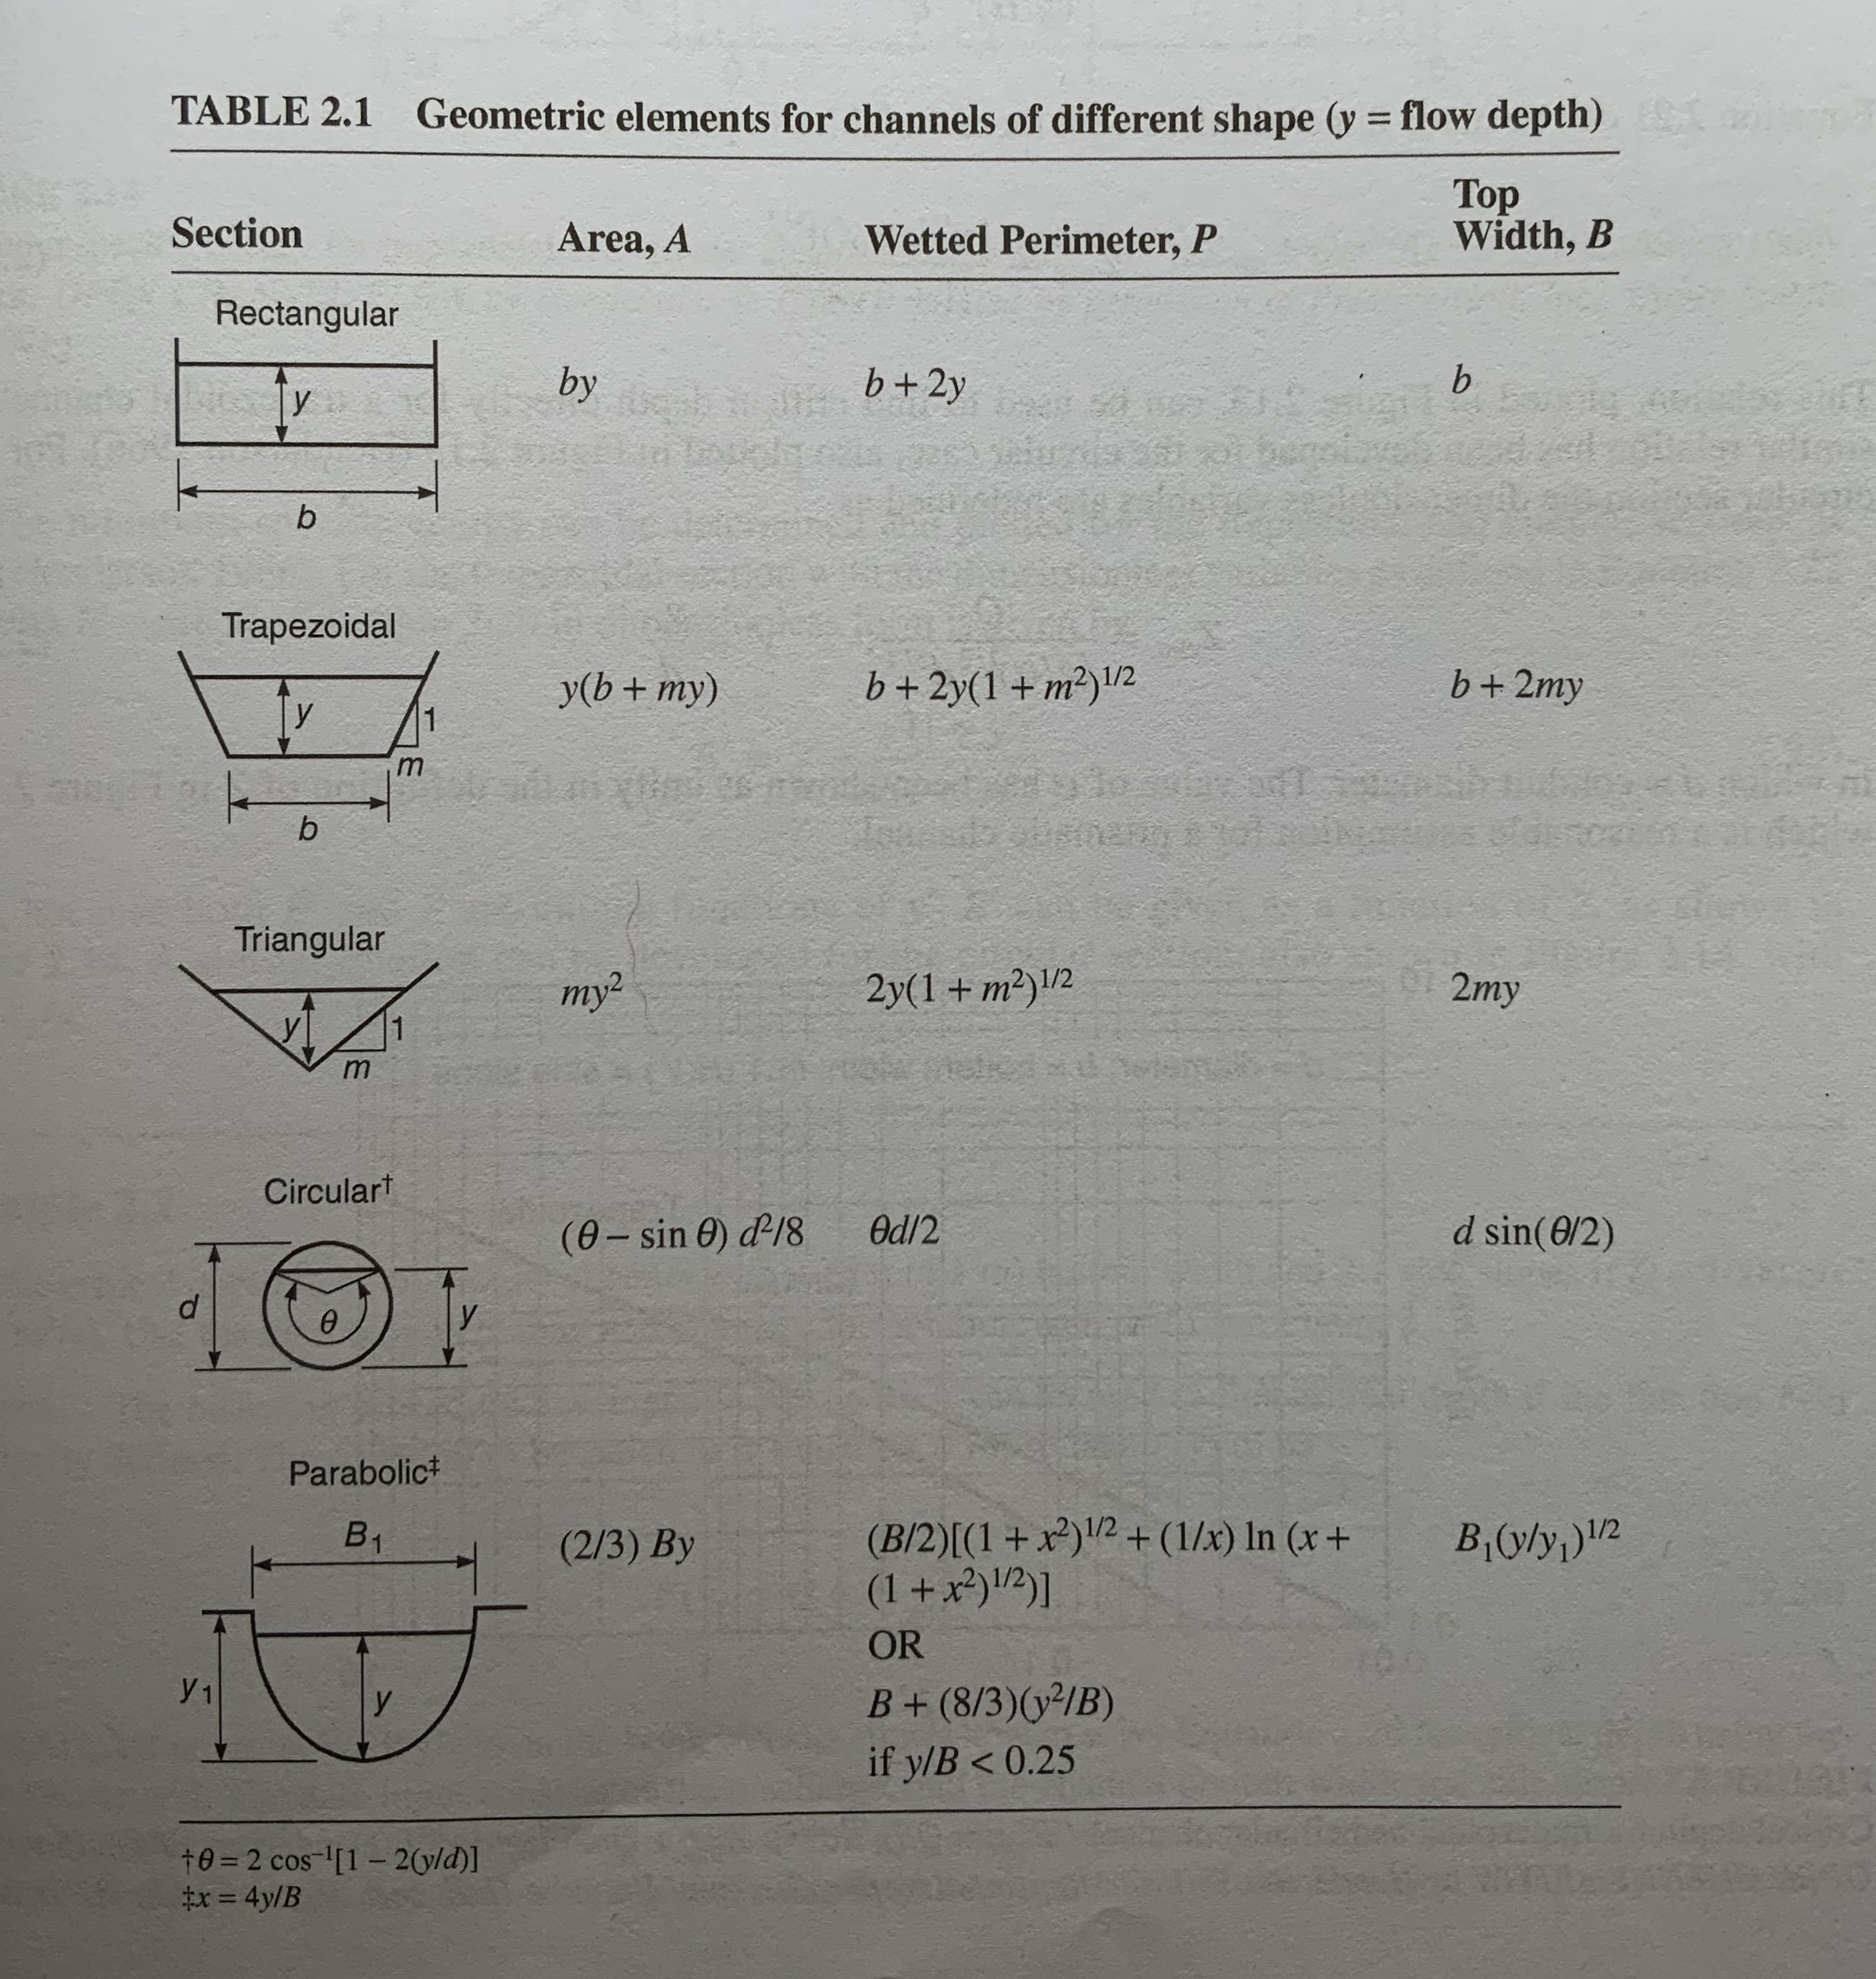
\includegraphics[width=0.9\textwidth]{sturm.jpg}
    \caption*{Source: \textit{Open Channel Hydraulics}, Third Edition, by Terry W. Sturm.}
\end{figure}

%%%%%%%%%%%%%%%%%%%%%%%%%%%%%%%%%%%%%%%%%%%%%%%%%%%%
% \newpage
% \question*{Creative Programming II}

% Submit your code to Gradescope as either \texttt{WordSearch.py} or \texttt{WordSearch.ipynb}.

%%%%%%%%%%%%%%%%%%%%%%%%%%%%%%%%%%%%%%%%%%%%%%%%%%%%
% \newpage
% \question{Creative programming}

% Write a Python program related to your engineering pursuits that demonstrates the use of \textbf{lists, dictionaries, and for loops}. Your program can be related to your other classes (past or present), research, job/internship, extracurriculars, or any other engineering topic. If you have an idea for a program topic but are unsure if it is appropriate, post on the Homework 1 page of the discussion board.

% Your program should demonstrate how functions can be used to decompose an engineering problem into sub-problems, and should be well-structured and well-documented. In addition to satisfying the requirements in the Style Guide, your program should meet the following requirements.

% \begin{itemize}
%     \item Use X amount of functions
%     \item Use at least one list
%     \item Use at least one dictionary
%     \item Use at least one for-loop and at least one list/dict comprehension
% \end{itemize}

% Additionally, your program should be able to run without requiring specialized hardware (e.g., connection to equipment that the instructor does not have access to). You are not restricted to the content we have covered; if you have Python experience and want to use content from later in the course or beyond, you may do so. As always, your code should follow the Style Guide: use descriptive variable and function names, include a docstring for each defined function, and include a short program summary. See the Style Guide for other guidelines and recommendations.

% Submit your program as a \texttt{.py} or \texttt{.ipynb} file to Gradescope. Submit any supporting files (e.g., data files) as well if applicable.

\end{document}

